\documentclass{article}

\usepackage[utf8x]{inputenc}
\usepackage[T1]{fontenc}
\usepackage[french]{babel}
\usepackage{xcolor}
\usepackage{listings}
\usepackage{mathptmx}
\usepackage{anyfontsize}
\usepackage{t1enc}
\usepackage[top=2cm, bottom=2cm, left=2cm, right=2cm]{geometry}
\usepackage{titlesec}
\usepackage{titling}
\usepackage[linesnumbered, french, frenchkw, onelanguage]{algorithm2e}
\usepackage{graphicx}
\usepackage{enumitem}
\usepackage[colorlinks = true,
            linkcolor = black,
            urlcolor  = black,
            citecolor = black,
            anchorcolor = black]{hyperref}

\newcommand{\changeurlcolor}[1]{\hypersetup{urlcolor=#1}}

\renewcommand\maketitlehooka{\null\mbox{}\vfill}
\renewcommand\maketitlehookd{\vfill\null}

\definecolor{codegreen}{rgb}{0,0.6,0}
\definecolor{codegray}{rgb}{0.5,0.5,0.5}
\definecolor{codepurple}{rgb}{0.58,0,0.82}
\definecolor{backcolour}{rgb}{0.95,0.95,0.92}
\definecolor{codekeywords}{rgb}{0.1,0.53,0.92}

\lstdefinestyle{c++}{
    backgroundcolor=\color{backcolour},   
    commentstyle=\color{codegreen},
    keywordstyle=\color{codekeywords},
    numberstyle=\tiny\color{codegray},
    stringstyle=\color{codepurple},
    basicstyle=\ttfamily\footnotesize,
    breakatwhitespace=false,         
    breaklines=true,                 
    captionpos=b,                    
    keepspaces=true,                 
    numbers=left,                    
    numbersep=5pt,                  
    showspaces=false,                
    showstringspaces=false,
    showtabs=false,                  
    tabsize=2,
    texcl=true,
    inputencoding=utf8,
    extendedchars=true,
    literate=
  {á}{{\'a}}1 {é}{{\'e}}1 {í}{{\'i}}1 {ó}{{\'o}}1 {ú}{{\'u}}1
  {Á}{{\'A}}1 {É}{{\'E}}1 {Í}{{\'I}}1 {Ó}{{\'O}}1 {Ú}{{\'U}}1
  {à}{{\`a}}1 {è}{{\`e}}1 {ì}{{\`i}}1 {ò}{{\`o}}1 {ù}{{\`u}}1
  {À}{{\`A}}1 {È}{{\'E}}1 {Ì}{{\`I}}1 {Ò}{{\`O}}1 {Ù}{{\`U}}1
  {ä}{{\"a}}1 {ë}{{\"e}}1 {ï}{{\"i}}1 {ö}{{\"o}}1 {ü}{{\"u}}1
  {Ä}{{\"A}}1 {Ë}{{\"E}}1 {Ï}{{\"I}}1 {Ö}{{\"O}}1 {Ü}{{\"U}}1
  {â}{{\^a}}1 {ê}{{\^e}}1 {î}{{\^i}}1 {ô}{{\^o}}1 {û}{{\^u}}1
  {Â}{{\^A}}1 {Ê}{{\^E}}1 {Î}{{\^I}}1 {Ô}{{\^O}}1 {Û}{{\^U}}1
  {œ}{{\oe}}1 {Œ}{{\OE}}1 {æ}{{\ae}}1 {Æ}{{\AE}}1 {ß}{{\ss}}1
  {ç}{{\c c}}1 {Ç}{{\c C}}1 {ø}{{\o}}1 {å}{{\r a}}1 {Å}{{\r A}}1
  {€}{{\EUR}}1 {£}{{\pounds}}1,
}
\lstset{style=c++}


\title{Outils d'aide à la décision TP3\\HVRP}
\author{Arquillière Mathieu - Zangla Jérémy}
%\date{\today}
%\date{\vspace{-5ex}}
\date{}

\begin{document}

\begin{titlepage}
  \maketitle
\end{titlepage}

\tableofcontents
\newpage
\listoffigures
\listofalgorithms
\newpage

\section{Introduction}
Notre problème ici est un problème de tournées de véhicules. Il faut trouver des algoritmes
nous rapprochant de solutions qui déterminent les tournées que doivent faire des véhicules
afin de livrer ou récupérer des marchandises chez des clients.

\section{Heuristiques de construction de solution}
Pour générer des solutions grâce à la fonction SPLIT qu'on détaillera plus loin, on a
besoin \emph{d'heuristiques de construction de solution initiales}. Celle-ci permettent
de générer un \emph{tour géant} à partir d'une instance d'un problème. Ce \emph{tour géant}
est un tableau contenant les sommets, les clients de l'instance, et selon l'ordre
de ce tableau, la fonction SPLIT générera une solution plus ou moins efficace. On
implémentera et testera 3 méthodes pour générer ce tour géant.

\subsection{Tour géant aléatoire}
\subsubsection{Principe}
Cette méthode consiste simplement à générer un tour géant aléatoirement. Il faut donc
créer un tableau d'une taille $n$ (nombre de sommets) contenant tous les nombres de
$1$ à $n$ répartis aléatoirement. Pour optimiser, on créé un tableau de la forme
$\forall i \in 1,...,n$ on a $T[i] = i$. On génére un indice $ind$ aléatoire et on insère
dans le tour géant $T[ind]$, puis on échange cet élément dans $T$ avec le dernier élément
et on réduit la taille du tableau de 1.

\subsubsection{Implémentation}
\begin{figure}[!ht]
  \centering
  \caption{Fonction de génération de tour géant - méthode aléatoire}
  \lstinputlisting[language=c++, firstline=141, lastline=162]{../ConsoleApplication1/ConsoleApplication1/hvrp.cpp}
\end{figure}


\subsection{Plus proche voisins}
\subsubsection{Principe}
Cette méthode pour générer le tour géant consiste à partir du sommet initial et de rajouter
au tour géant son voisin le plus proche, ensuite on rajoute le voisin le plus proche à
ce voisin etc. Cette méthode s'est révélée beaucoup plus efficace que la méthode précédente.
\newpage
\subsubsection{Implémentation}
\begin{figure}[!ht]
  \centering
  \caption{Fonction de génération de tour géant - méthode aléatoire}
  \lstinputlisting[language=c++, firstline=187, lastline=232]{../ConsoleApplication1/ConsoleApplication1/hvrp.cpp}
\end{figure}

\subsection{Plus proche voisins randomisés}
\subsubsection{Principe}
Cette méthode consiste à prendre les 5 plus proches voisins du sommet initial et de choisir
aléatoirement dans ces sommets lequel on ajoute dans le tour géant. Cependant l'aléatoire
n'est pas uniforme. En effet, on trie ces 5 sommets (en fonction de la distance avec le
sommet initial) et le premier de cette liste à 80\% de chance d'être séléctionné. Puis, le
deuxième, lui, à 80\% de chance des 20\% restants d'être séléctionné, etc. Une fois le
sommet choisi, on ré-exécute le même algorithme sur lui et on itère de cette façon jusqu'à
avoir tous les sommets dans le tour géant.

\newpage
\subsubsection{Implémentation}
\begin{figure}[!ht]
  \centering
  \caption{PPVR - 5 plus proches voisins}
  \lstinputlisting[language=c++, firstline=233, lastline=277]{../ConsoleApplication1/ConsoleApplication1/hvrp.cpp}
\end{figure}
\begin{figure}[!ht]
  \centering
  \caption{PPVR - boucle de choix dans les 5 plus proches voisins}
  \lstinputlisting[language=c++, firstline=279, lastline=307]{../ConsoleApplication1/ConsoleApplication1/hvrp.cpp}
\end{figure}

\newpage
\section{Grasp}
Lorsqu'on obtient une solution à partir d'un tour géant (cf. SPLIT), on obtient un certain
nombre de tournées avec chacune un véhicule et un coût. La somme de ces coûts donnent le
coût total de la solution.

Le but du grasp est d'améliorer une solution, pour ça on se sert de différents
\emph{opérateurs} qui peuvent améliorer chacun la solution avec des manières différentes.
Lorsque un \emph{opérateurs} améliore la solution, sa probabilité d'etre utilisé dans le grasp augmente, et inversement si il échoue sa probabilité augmente.
\subsection{Opérateur 2OPT}
\subsubsection{Principe}
Cet opérateur consiste à parcourir chaque tournée et essayer d'inverser l'ordre de deux
sommets dans cette tournée. Si cette inversion est possible (le volume de la tournée est
transportable par le véhicule) et qu'elle améliore le coût, alors on l'effectue.

\subsubsection{Algorithme}
\begin{algorithm}[H]
  \For{$i = 0$ \KwTo $nb\_tournees$}
  {
    T $\leftarrow$ Tournées[$i$]\;
    \For{$a = 1$ \KwTo $T.nb\_sommets - 3$}
    {
      \For{$b = a$ \KwTo $T.nb\_sommets - 2$}
      {
        x $\leftarrow$ T[$a$]\;
        y $\leftarrow$ T[$b$]\;
        m $\leftarrow$ Distance($x - 1$, $x$) + Distance($x$, $y$) + Distance($y$, $y + 1$)\;
        p $\leftarrow$ Distance($x - 1$, $y$) + Distance($y$, $x$) + Distance($x$, $y + 1$)\; 
 
        \If{$m > p$}
        {
          Echange\_Entre($a$, $b$)\;
          Mettre à jour le cout de la tournée\;
          Mettre à jour le cout de la solution\;
          \Return Vrai\;
        }
      }
    }
  }
  \Return Faux\;
  \caption{Algorithme 2OPT}
\end{algorithm}

\subsection{Opérateur 2OPT inter-tournée}
\subsubsection{Principe}
Cet opérateur consiste à parcourir les tournées d'une solution et à chaque itération, en avoir
deux pour tester de transformer ces deux tournées. Le but est de parcourir les sommets de
ces deux tournées et d'essayer, lorsque ça diminue le coût, de transformer la 1ere tournée
avec son début et la fin de l'autre tournée et inversement.

\begin{figure}[!ht]
  \caption{Représentation graphique de l'opérateur 2OPT inter-tournée}
  \centering
  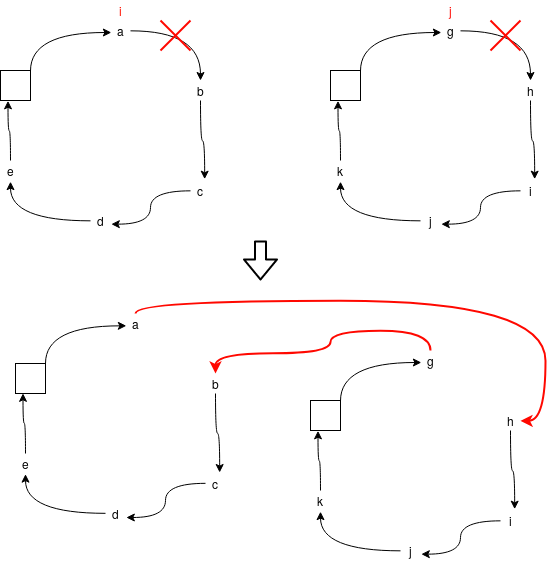
\includegraphics[scale=0.60]{images/inter-tournee.png}
\end{figure}

\newpage
\subsubsection{Algorithme}
\begin{algorithm}[H]
  \For{$i = 0$ \KwTo $nb\_tournees - 2$}
  {
    T1 $\leftarrow$ Tournées[$i$]\;
    \For{$j = i + 1$ \KwTo $nb\_tournees - 1$}
    {
      debut\_t1 $\leftarrow$ = 0\;
      T2 $\leftarrow$ Tournées[$j$]\;
      \For{$a = 1$ \KwTo $T1.nb\_sommets - 2$}
      {
        debut\_t2 $\leftarrow$ = 0\;
        debut\_t1 += Distance(T1[$a - 1$], T1[$a$])\;
        \For{$b = 1$ \KwTo $T2.nb\_sommets - 2$}
        {
          debut\_t1 += Distance(T1[$b - 1$], T2[$b$])\;

          passage\_a\_b $\leftarrow$ Distance(T1[$a$], T2[$b + 1$])\;
          passage\_b\_a $\leftarrow$ Distance(T1[$b$], T2[$a + 1$])\;

          fin\_t1 $\leftarrow$ T1.distance - $debut\_t1$ - Distance(T1[$a$], T1[$a + 1$])\;
          fin\_t2 $\leftarrow$ T2.distance - $debut\_t2$ - Distance(T2[$b$], T2[$b + 1$])\;

          distance\_total\_t1 $\leftarrow$ $debut\_t1$ + $passage\_a\_b$ + $fin\_t2$\;
          distance\_total\_t2 $\leftarrow$ $debut\_t2$ + $passage\_b\_a$ + $fin\_t1$\;
          
          \If{$distance\_total\_t1 + distance\_totatl\_t2 < T1.distance + T2.distnce$}
          {
            Echange\_A\_Partir\_De($a$, $b$)\;
            Mettre à jour le cout des tournée\;
            Mettre à jour le cout de la solution\;
            \Return Vrai\;
          }
        }
      }
    }
  }
  \Return Faux\;
  \caption{Algorithme 2OPT inter-tournée}
\end{algorithm}

\subsection{Opérateur insertion}
\subsubsection{Principe}
Cet opérateur consiste à parcourir les tournées d'une solution et de prendre 2 tournées
de la même façon que l'opérateur 2OPT inter-tournée. La différence est que lui essaye
de retirer un sommet de la première tournée et de l'insérer dans la deuxième à tous les
endroits possibles.

\subsubsection{Algorithme}
\begin{algorithm}[H]
  \For{$i = 0$ \KwTo $nb\_tournees - 1$}
  {
    T1 $\leftarrow$ Tournées[$i$]\;
    \For{$j = 0$ \KwTo $nb\_tournees - 1$}
    {
      \If{$i \ne j$}
      {
        \If{$T1.nb\_sommets == 3$}
        {
          \For{$b = 0$ \KwTo $T2.nb\_sommets - 1$}
          {
            cout\_t2 $\leftarrow$ T2.cout + T2.cout\_modulaire * (Distance(T2[$b$], T1[$a$]) + Distance(T1[$a$], T2[$b + 1$]) - Distance(T2[$b$], T2[$b + 1$]))\;
            \If{$cout\_t2 < T1.cout + T2.cout$}
            {
              Insertion($a$)\;
              Mettre à jour le cout de la tournée T2\;
              Suppression de la tournée T1\;
              Mettre à jour le cout de la solution\;
              \Return Vrai\;
            }
          }
        }
        \Else
        {
          \For{$a = 1$ \KwTo $T1.nb\_sommets - 1$}
          {
            \For{$b = 0$ \KwTo $T2.nb\_sommets - 1$}
            {
              m $\leftarrow$ Distance(T1[$a - 1$], T1[$a$]) + Distance(T1[$a$], T1[$a + 1$]) + Distance(T2[$b$], T2[$b + 1$])\;
              p $\leftarrow$ Distance(T2[$b$], T1[$a$]) + Distance(T1[$a$], T2[$b + 1$]) + Distance(T1[$a - 1$], T1[$a + 1$])\;
              \If{$m > p$}
              {
                Insertion($a$)\;
                Mettre à jour le cout des tournée\;
                Mettre à jour le cout de la solution\;
                \Return Vrai\;
              }
            }
          }
        }
      }
    }
  }
  \Return Faux\;
  \caption{Algorithme OPT Insertion}
\end{algorithm}
\end{document}
